\documentclass[]{article}
\newcommand{\FileDepth}{../../..}
\usepackage[letterpaper, landscape, margin=0.5cm]{geometry}
\usepackage[T1]{fontenc}
\usepackage{textcomp}%Not strictly necessary, but gives \textmu command for "micro."
\usepackage{fancyhdr}
\usepackage{amsmath}
\usepackage{amssymb}
\usepackage{graphicx}
\usepackage{xcolor}
\usepackage{tikz}
\usetikzlibrary{calc}
\usepackage[shortlabels]{enumitem}
\usepackage{multicol}
\usepackage{vwcol}
\usepackage{hyperref}
\usepackage{wrapfig}
%opening
\newcommand{\SecType}{L}
\newcommand{\Week}{18}
\title{PH 211 Lecture \Week}
\author{Benjamin Bauml}
\date{Summer 2024}

\newcommand{\Purpose}{4}
\newcommand{\DefOnly}{0}

\input{\FileDepth/Formats/Assignment20240614.tex}
\usepackage[absolute]{textpos}
% This package relies on Assignment Format 2024-06-14 or later to work. It is recommended that the Purpose and DefOnly commands be given as such:
%\newcommand{\Purpose}{4}
%\newcommand{\DefOnly}{0}
% Activities need to be entered outside of the TeacherMargin and PresentSpace environments, otherwise they will be defined only locally. They can even go in the preamble.
\newenvironment{TeacherMargin}{\begin{textblock*}{10.8cm}(0.5cm,0.5cm)
\small}{\end{textblock*}
\hspace{0.1cm}}
\newenvironment{PresentSpace}{\begin{textblock*}{0.3cm}(26.85cm,9.35cm)
--
\end{textblock*}
\begin{textblock*}{15.6cm}(11.8cm,0.5cm)
\begin{Repurpose}{1}
\Large}{\end{Repurpose}
\end{textblock*}
\hspace{0.1cm}}

%\newcommand{\FBDaxes}[4][2]{
	\begin{scope}[shift={(#2)},rotate=#3]
		% x-axis
		\draw[thick,->] (-#1,0) -- (#1,0);
		\node[anchor=west] at (#1,0) {$x$};
		% y-axis
		\draw[thick,->] (0,-#1) -- (0,#1);
		\node[anchor=south] at (0,#1) {$y$};
		\coordinate (#4) at (0,0);
	\end{scope}
}
\newcommand{\FBDvectorMA}[4]{
	\begin{scope}[shift={(#1)}]
		\coordinate (#4tip) at ({#2*cos(#3)},{#2*sin(#3)});
		\draw[ultra thick,blue,->] (#1) -- (#4tip);
	\end{scope}
}
\newcommand{\FBDvectorXY}[3]{
	\begin{scope}[shift={(#1)}]
		\coordinate (#3tip) at (#2);
		\draw[ultra thick,blue,->] (0,0) -- (#3tip);
	\end{scope}
}
\newcommand{\FBDdot}[1]{
	\filldraw[black] (#1) circle (3pt);
}
\newcommand{\FBDbox}[5][1]{
	\begin{scope}[shift={(#2)},rotate=#3]
		\filldraw[color=black,fill=white,thick] ({-#1/2},{#1/2}) -- ({-#1/2},{-#1/2}) -- ({#1/2},{-#1/2}) -- ({#1/2},{#1/2}) -- cycle;
		% Left side coordinates
		\coordinate (#4ltq) at ({-#1/2},{#1/4});
		\coordinate (#4lcent) at ({-#1/2},0);
		\coordinate (#4lbq) at ({-#1/2},{-#1/4});
		% right side coordinates
		\coordinate (#4rtq) at ({#1/2},{#1/4});
		\coordinate (#4rcent) at ({#1/2},0);
		\coordinate (#4rbq) at ({#1/2},{-#1/4});
		% top coordinates
		\coordinate (#4tlq) at ({-#1/4},{#1/2});
		\coordinate (#4tcent) at (0,{#1/2});
		\coordinate (#4trq) at ({#1/4},{#1/2});
		% bottom coordinates
		\coordinate (#4blq) at ({-#1/4},{-#1/2});
		\coordinate (#4bcent) at (0,{-#1/2});
		\coordinate (#4brq) at ({#1/4},{-#1/2});
		% corners
		\coordinate (#4tl) at ({-#1/2},{#1/2});
		\coordinate (#4tr) at ({#1/2},{#1/2});
		\coordinate (#4bl) at ({-#1/2},{-#1/2});
		\coordinate (#4br) at ({#1/2},{-#1/2});
		\node at (0,0) {#5};
	\end{scope}
}
%\newcommand{\MVec}[3][0]{%Creates a momentum vector of length #3 centered at #2 and rotated #1 degrees counterclockwise.
	\begin{scope}[rotate=#1,shift={(#2)}]
		\draw[->,thick] ({-#3/2},0) -- ({#3/2},0);
	\end{scope}
}
\newcommand{\MDot}[1]{%Creates a dot at #1 to represent a zero vector.
	\filldraw (#1) circle (1pt);
}
\newcommand{\MVDRows}[2][4.5]{%Creates the rows (initial, delta, final) of a momentum vector diagram. The optional argument determines the width of the table, and defaults to a good length for three columns (two objects and the total system). The non-optional argument gives a coordinate name (not displayed) to the diagram.
	\begin{scope}
		%\draw[thick] (0,5.5) -- (0,0);
		\draw[thick] (-1,4.5) -- (#1,4.5);
		\node at (-0.5,3.75) {$\vec{p}_{i}$};
		\draw[thick] (-1,3) -- (#1,3);
		\node at (-0.5,2.25) {$\Delta\vec{p}$};
		\draw[thick] (-1,1.5) -- (#1,1.5);
		\node at (-0.5,0.75) {$\vec{p}_{f}$};
		\coordinate (#2) at (0,5);
	\end{scope}
}
\newcommand{\MVDCol}[4][0.75]{%Creates a column for an object in a momentum vector diagram. The first (non-optional) argument is the coordinate name (not displayed) of the column, while the second is the displayed column header. The first argument also names the three entries down the column. The third argument anchors the column, so it should either be the coordinate name of the MVD (for the first column) or the coordinate name of the previous column. The optional argument indicates how far the center of the column should be from the previous column's edge, and defaults to 0.75.
	\begin{scope}[shift={(#4)}]
		\node at (#1,0) {#3};
		%\draw[thick] ({#1*2},0.5) -- ({#1*2},-5);
		\draw[thick] (0,0.5) -- (0,-5);
		\coordinate (#2init) at (#1,-1.25);
		\coordinate (#2delt) at (#1,-2.75);
		\coordinate (#2fin) at (#1,-4.25);
		\coordinate (#2) at ({#1*2},0);
	\end{scope}
}

%\input{\FileDepth/Activities/Activity_One/Activity_One.tex}
%\input{\FileDepth/Activities/Activity_Two/Activity_Two.tex}

\begin{document}
\begin{TeacherMargin}
\noindent Recall that force is the negative derivative of the potential energy:
\[
\vec{F} = -\frac{dU}{dx}\hat{x}.
\]
As such, the largest force occurs where the slope is steepest. This appears to happen at about $x=6.8$ m (where the slope is positive, and therefore the force is pointing in the negative direction) and close to $x=3$ m (where the slope is negative, and therefore the force is pointing in the positive direction).
\end{TeacherMargin}
\begin{PresentSpace}
\begin{center}
	\huge Lecture \Week: Potential Energy Diagrams
\end{center}
\vspace{0.5cm}
\underline{Warm-Up Activity} \\
A potential energy diagram \\
for some system is shown \\
at right. At what position(s) \\
is the magnitude of the force \\
at a maximum?
\end{PresentSpace}
\begin{textblock*}{8cm}(18cm,1.2cm)
\begin{center}
	\Large
	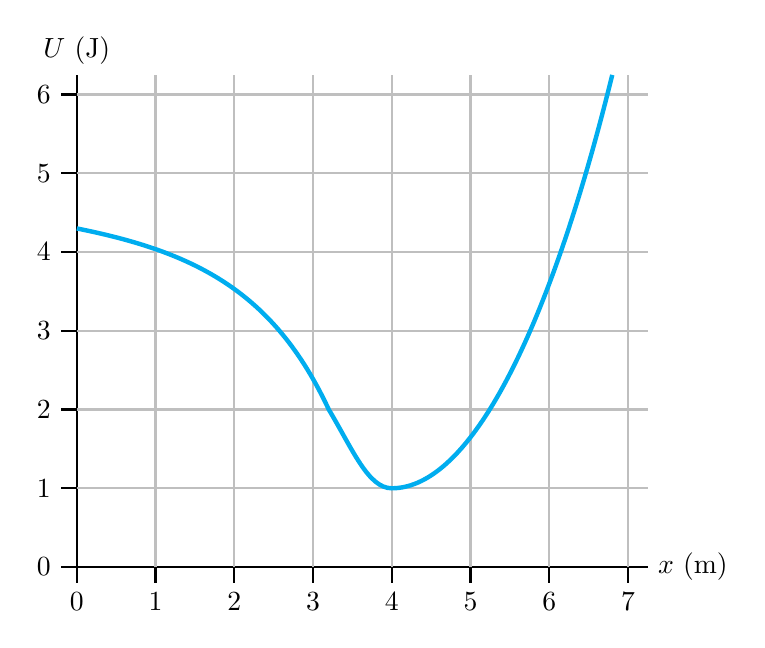
\begin{tikzpicture}
		\draw[thick] (0,-0.2) node[anchor=north] {0} -- (0,6.25) node[anchor=south] {$U$ (J)};
		\foreach \y in {1,2,3,4,5,6}
			\draw[thick] (-0.2,\y) node[anchor=east] {\y} -- (0,\y);
		\foreach \y in {1,2,3,4,5,6}
			\draw[thick,lightgray] (0,\y) -- (7.25,\y);
		\draw[thick] (-0.2,0) node[anchor=east] {0} -- (7.25,0) node[anchor=west] {$x$ (m)};
		\foreach \x in {1,2,3,4,5,6,7}
			\draw[thick] (\x,-0.2) node[anchor=north] {\x} -- (\x,0);
		\foreach \x in {1,2,3,4,5,6,7}
			\draw[thick,lightgray] (\x,0) -- (\x,6.25);
		\draw[ultra thick,cyan] (0,4.3) .. controls (1.5,4) and (2.5,3.5) .. (3.2,2) .. controls (3.5,1.5) and (3.7,1) .. (4,1) .. controls (5,1) and (6,3) .. (6.8,6.25);
	\end{tikzpicture}
\end{center}
\end{textblock*}
\newpage
\begin{TeacherMargin}

\end{TeacherMargin}
\begin{PresentSpace}
\vspace{-10pt}
\section*{A Deeper Model for Interactions}
\vspace{-10pt}
\begin{itemize}
	\item Quantities
	\begin{itemize}
		\item Energy \qquad \qquad \qquad \quad \ \ $E$
		\item Work \qquad \qquad \qquad \quad \ \ \ \ $W = \int_{r_{i}}^{r_{f}}\vec{F}\cdot d\vec{r}$
		\item Kinetic Energy \qquad \qquad $K=\frac{1}{2}mv^{2}$
		\item Potential Energy \qquad \quad \ $U=$ depends on interaction \\
		You have to tell everyone where zero $PE$ is!
		\begin{itemize}
			\item Gravity \qquad $U_{g} = mgy$
			\item Spring \qquad \ $U_{sp} = \frac{1}{2}kx^{2}$
		\end{itemize}
	\end{itemize}
	\item Laws
	\begin{itemize}
		\item Work-energy theorem \quad $W_{\text{net,ext}} = \Delta E_{\text{total}}$
	\end{itemize}
\end{itemize}
\end{PresentSpace}
\newpage
\begin{TeacherMargin}
\begin{center}
	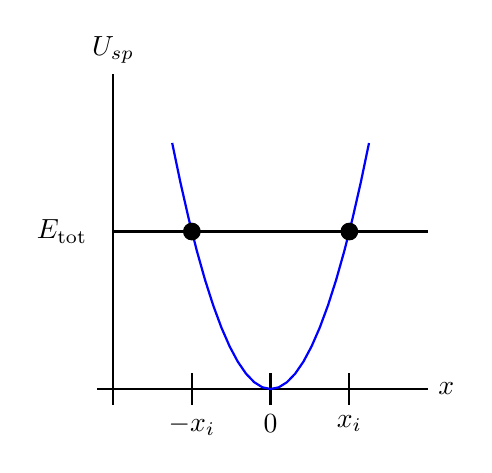
\begin{tikzpicture}
		\draw[thick] (-2,-0.2) -- (-2,4) node[anchor=south] {$U_{sp}$};
		\draw[thick] (-2.2,0) -- (2,0) node[anchor=west] {$x$};
		\draw[thick] (-1,0.2) -- (-1,-0.2) node[anchor=north] {$-x_{i}$};
		\draw[thick] (0,0.2) -- (0,-0.2) node[anchor=north] {$0$};
		\draw[thick] (1,0.2) -- (1,-0.2) node[anchor=north] {$x_{i}$};
		\draw[thick,blue,domain=-1.25:1.25,variable=\x] plot (\x,2*\x*\x);
		\draw[thick] (-2,2) node[anchor=east,shift={(-0.2,0)}] {$E_{\text{tot}}$} -- (2,2);
		\foreach \x in {-1,1}
			\filldraw (\x,2) circle (3pt);
	\end{tikzpicture}
\end{center}
The spring is stretched when $x>0$ and compressed when $x<0$. The potential energy is largest at maximum stretch or compression ($\pm x_{i}$ in this particular case), and it is smallest (zero) when the spring is at its equilibrium length ($x=0$). These things can be directly read off of the graph. \\

\noindent The total energy of the block-and-spring system stays the same, as there are no external forces that do work (which we will get into more on Monday). Energy in the system is converted back and forth between kinetic and potential energy without loss or gain. We represent this on the graph with a horizontal line for total energy. \\

\noindent We know $E_{\text{total}} = K+U_{sp}$, so $K = E_{\text{total}}-U_{sp}$. When potential energy is at a minimum, kinetic energy is at a maximum, and vice versa. We have the most kinetic energy at the equilibrium length ($x=0$), and the least (zero kinetic energy) when the spring is at maximum stretch or compression (which makes sense, as if the spring had any kinetic energy left when it reached one of these end points, it would be able to continue moving and reach a farther point from equilibrium). \\

\noindent The spring force is largest when potential energy is highest (because we are at maximum stretch), and smallest at $x=0$ (where the spring is unstretched and potential energy is zero). This can be seen from the slope of the graph, as $\vec{F}^{sp} = -\frac{dU_{sp}}{dx}\hat{x}$.
\end{TeacherMargin}
\begin{PresentSpace}
\vspace{-10pt}
\section*{L\Week-1: Potential Energy Diagrams}
\vspace{-5pt}
The potential energy of the spring is given by $U_{sp} = \frac{1}{2}kx^{2}$.
\begin{itemize}
	\item Sketch a potential energy diagram \\
	(a graph of $U_{sp}$ vs. $x$).
	\item Where is the potential energy \\
	largest? Smallest? How can you tell?
	\item How does the total energy change? \\
	How can you tell?
	\item Where is the kinetic energy largest? \\
	Smallest? How can you tell?
	\item Where is the spring force largest? Smallest? How can you tell?
\end{itemize}
\end{PresentSpace}
\begin{textblock*}{5cm}(20cm,2.5cm)
\begin{center}
	\Large
	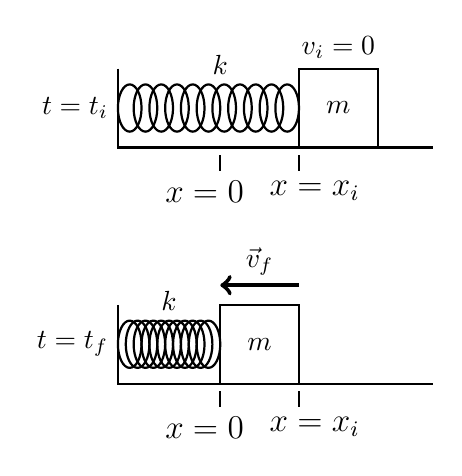
\begin{tikzpicture}
		\begin{scope}[shift={(0,-3)}]
			\node[anchor=east] at (0,0.5) {$t=t_{f}$};
			\draw[thick] (0,1) -- (0,0) -- (4,0);
			\foreach \s in {0,1,2,3,4,5,6,7,8,9,10}
			\draw[thick] (\s*0.1+0.15,0.5) circle (0.15 and 0.3);
			\node[anchor=south] at (0.65,0.8) {$k$};
			\draw[thick,shift={(1.3,0)}] (0,0) -- (0,1) -- (1,1) -- (1,0) -- cycle;
			\node at (1.8,0.5) {$m$};
			\draw[ultra thick,<-,shift={(1.3,0)}] (0,1.25) -- (0.5,1.25) -- (1,1.25);
			\node[anchor=south] at (1.8,1.25) {$\vec{v}_{f}$};
			\draw[thick] (1.3,-0.1) -- (1.3,-0.3) node[anchor=north,shift={(-0.2,0)}] {\large$x=0$};
			\draw[thick] (2.3,-0.1) -- (2.3,-0.3) node[anchor=north,shift={(0.2,0)}] {\large$x=x_{i}$};
		\end{scope}
		\begin{scope}[shift={(0,0)}]
			\node[anchor=east] at (0,0.5) {$t=t_{i}$};
			\draw[thick] (0,1) -- (0,0) -- (4,0);
			\foreach \s in {0,1,2,3,4,5,6,7,8,9,10}
			\draw[thick] (\s*0.2+0.15,0.5) circle (0.15 and 0.3);
			\node[anchor=south] at (1.3,0.8) {$k$};
			\draw[thick,shift={(2.3,0)}] (0,0) -- (0,1) -- (1,1) -- (1,0) -- cycle;
			\node at (2.8,0.5) {$m$};
			\node[anchor=south] at (2.8,1) {$v_{i}=0$};
			\draw[thick] (1.3,-0.1) -- (1.3,-0.3) node[anchor=north,shift={(-0.2,0)}] {\large$x=0$};
			\draw[thick] (2.3,-0.1) -- (2.3,-0.3) node[anchor=north,shift={(0.2,0)}] {\large$x=x_{i}$};
		\end{scope}
	\end{tikzpicture}
\end{center}
\end{textblock*}
\newpage
\begin{TeacherMargin}
\noindent As $y$ increases, the potential energy increases (it becomes less negative). We expect to store more potential energy in the gravitational field when we move farther from the surface (more kinetic energy will be gained in a fall from a greater height). \\

\noindent The strange part is that the energy is entirely negative, and the zero of potential energy is out at $y=\infty$. In orbital mechanics, it is actually convenient to have the energy near a planet be negative, as that tells you how much energy an object needs to escape the planet's gravity. In this case, if we give the astronaut at least 6.2 GJ of kinetic energy, they will be able to get arbitrarily far away from the planet without running out of speed and falling back to the surface. \\

\noindent The force is the negative slope of the potential energy: $\vec{F} = -\frac{dU}{dy}\hat{y}$ (the slope is positive everywhere, so the force always points back toward Earth). The slope decreases as we get farther from the surface, indicating that the force of gravity decreases in magnitude. We expect the force of gravity to get weaker as we get farther away from a gravitating body.
\end{TeacherMargin}
\begin{PresentSpace}
\vspace{-10pt}
\section*{L\Week-2: Astronaut Energy I}
\vspace{-5pt}
We send an astronaut into space, creating the following graph of potential energy $U_{g}$ vs. distance from the surface of the Earth $y$.
\begin{itemize}
	\item Describe how the potential \\
	energy of the system changes \\
	as $y$ increases. Do you think \\
	this behavior makes sense?
	\item Describe how the \\
	gravitational force changes \\
	as $y$ increases. Do you think \\
	this behavior makes sense? (\textbf{Hint:} What \\
	feature of the graph tells you about the force?)
\end{itemize}
\end{PresentSpace}
\begin{textblock*}{7.5cm}(19cm,2.7cm)
\begin{center}
	\normalsize
	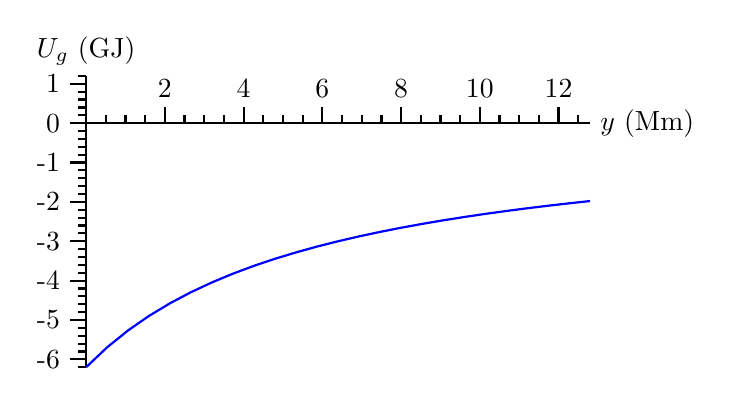
\begin{tikzpicture}
		\draw[thick] (0,-3.1) -- (0,0.6) node[anchor=south] {$U_{g}$ (GJ)};
		\foreach \y in {0.6,0.4,0.3,0.2,0.1,-0.1,-0.2,-0.3,-0.4,-0.6,-0.7,-0.8,-0.9,-1.1,-1.2,-1.3,-1.4,-1.6,-1.7,-1.8,-1.9,-2.1,-2.2,-2.3,-2.4,-2.6,-2.7,-2.8,-2.9,-3.1}
			\draw[thick] (-0.1,\y) -- (0,\y);
		\foreach \y in {1,0,-1,-2,-3,-4,-5,-6}
			\draw[thick] (-0.2,\y/2) node[anchor=east] {\y} -- (0,\y/2);
		\draw[thick] (0,0) -- (6.4,0) node[anchor=west] {$y$ (Mm)};
		\foreach \x in {0.25,0.5,0.75,1.25,1.5,1.75,2.25,2.5,2.75,3.25,3.5,3.75,4.25,4.5,4.75,5.25,5.5,5.75,6.25}
			\draw[thick] (\x,0.1) -- (\x,0);
		\foreach \x in {2,4,6,8,10,12}
			\draw[thick] (\x/2,0.2) node[anchor=south] {\x} -- (\x/2,0);
		%\draw[thick,gray] (0,-1) -- (6.4,-1);% Guide line
		%\draw[thick,blue,domain=0:6.4,variable=\r] plot (\r,{-(6.4*3.1)/(6.4+\r)});% Uses actual Earth radius.
		\draw[thick,blue,domain=0:6.4,variable=\r] plot (\r,{-(3*3.1)/(3+\r)});% Uses less than half of Earth's radius.
	\end{tikzpicture}
\end{center}
\end{textblock*}
\newpage
\begin{TeacherMargin}
\begin{center}
	\normalsize
	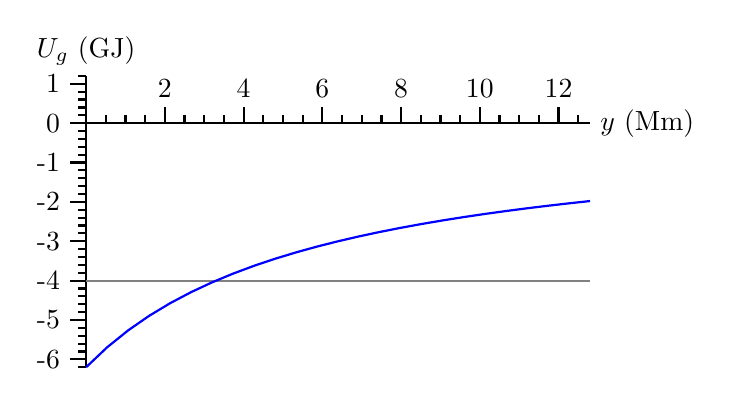
\begin{tikzpicture}
		\draw[thick] (0,-3.1) -- (0,0.6) node[anchor=south] {$U_{g}$ (GJ)};
		\foreach \y in {0.6,0.4,0.3,0.2,0.1,-0.1,-0.2,-0.3,-0.4,-0.6,-0.7,-0.8,-0.9,-1.1,-1.2,-1.3,-1.4,-1.6,-1.7,-1.8,-1.9,-2.1,-2.2,-2.3,-2.4,-2.6,-2.7,-2.8,-2.9,-3.1}
		\draw[thick] (-0.1,\y) -- (0,\y);
		\foreach \y in {1,0,-1,-2,-3,-4,-5,-6}
		\draw[thick] (-0.2,\y/2) node[anchor=east] {\y} -- (0,\y/2);
		\draw[thick] (0,0) -- (6.4,0) node[anchor=west] {$y$ (Mm)};
		\foreach \x in {0.25,0.5,0.75,1.25,1.5,1.75,2.25,2.5,2.75,3.25,3.5,3.75,4.25,4.5,4.75,5.25,5.5,5.75,6.25}
		\draw[thick] (\x,0.1) -- (\x,0);
		\foreach \x in {2,4,6,8,10,12}
		\draw[thick] (\x/2,0.2) node[anchor=south] {\x} -- (\x/2,0);
		\draw[thick,gray] (0,-2) -- (6.4,-2);% Guide line
		%\draw[thick,blue,domain=0:6.4,variable=\r] plot (\r,{-(6.4*3.1)/(6.4+\r)});% Uses actual Earth radius. Actual max height would be 7 Mm, not the 3.5 Mm from using the other line.
		\draw[thick,blue,domain=0:6.4,variable=\r] plot (\r,{-(3*3.1)/(3+\r)});% Uses less than half of Earth's radius.
	\end{tikzpicture}
\end{center}
Since $E_{\text{total}} = -4$ GJ, and $E_{\text{total}} = K + U_{g}$, we know that the astronaut stops when the potential energy is equal to the total energy (meaning there is no kinetic energy, and the astronaut has stopped ascending). This occurs at approximately $y=3.5$ Mm above the planet's surface. \\

\noindent The largest kinetic energy occurs when the potential energy is smallest, which happens to be at the surface of the Earth. When $y=0$ Mm, $U_{g} = -6.2$ GJ, and therefore
\[
K=E-U_{g} = -4\text{ GJ} - (-6.2\text{ GJ}) = 2.2\text{ GJ}.
\]
\end{TeacherMargin}
\begin{PresentSpace}
\vspace{-10pt}
\section*{L\Week-3: Astronaut Energy II}
\vspace{-5pt}
We send an astronaut into space, creating the following graph of potential energy $U_{g}$ vs. distance from the surface of the Earth $y$. \\

\noindent Assume the total energy of the \\
Astronaut-Earth system is $-4$ GJ.
\begin{itemize}
	\item How high above the surface \\
	of the Earth does the \\
	astronaut go?
	\item What is the astronaut's \\
	largest kinetic energy? \\
	Where does this happen?
\end{itemize}
\end{PresentSpace}
\begin{textblock*}{7.5cm}(19cm,2.7cm)
\begin{center}
	\normalsize
	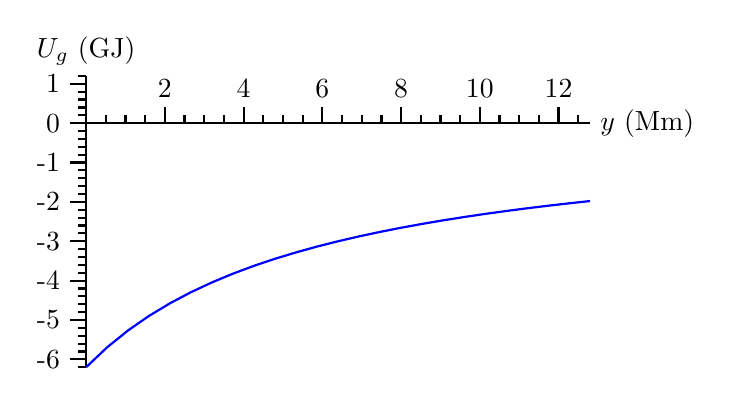
\begin{tikzpicture}
		\draw[thick] (0,-3.1) -- (0,0.6) node[anchor=south] {$U_{g}$ (GJ)};
		\foreach \y in {0.6,0.4,0.3,0.2,0.1,-0.1,-0.2,-0.3,-0.4,-0.6,-0.7,-0.8,-0.9,-1.1,-1.2,-1.3,-1.4,-1.6,-1.7,-1.8,-1.9,-2.1,-2.2,-2.3,-2.4,-2.6,-2.7,-2.8,-2.9,-3.1}
		\draw[thick] (-0.1,\y) -- (0,\y);
		\foreach \y in {1,0,-1,-2,-3,-4,-5,-6}
		\draw[thick] (-0.2,\y/2) node[anchor=east] {\y} -- (0,\y/2);
		\draw[thick] (0,0) -- (6.4,0) node[anchor=west] {$y$ (Mm)};
		\foreach \x in {0.25,0.5,0.75,1.25,1.5,1.75,2.25,2.5,2.75,3.25,3.5,3.75,4.25,4.5,4.75,5.25,5.5,5.75,6.25}
		\draw[thick] (\x,0.1) -- (\x,0);
		\foreach \x in {2,4,6,8,10,12}
		\draw[thick] (\x/2,0.2) node[anchor=south] {\x} -- (\x/2,0);
		%\draw[thick,gray] (0,-2) -- (6.4,-2);% Guide line
		%\draw[thick,blue,domain=0:6.4,variable=\r] plot (\r,{-(6.4*3.1)/(6.4+\r)});% Uses actual Earth radius.
		\draw[thick,blue,domain=0:6.4,variable=\r] plot (\r,{-(3*3.1)/(3+\r)});% Uses less than half of Earth's radius.
	\end{tikzpicture}
\end{center}
\end{textblock*}
\newpage
\begin{TeacherMargin}
	
\end{TeacherMargin}
\begin{PresentSpace}
\section*{Main Ideas}
\begin{itemize}
	\item The work-energy theorem can be used to solve a broad array of problems.
	\item A variety of representations can be helpful in solving problems using work and energy.
\end{itemize}
\end{PresentSpace}
\end{document}